\documentclass[a4paper, 12pt, conference]{IEEEtran}
\usepackage[utf8]{inputenc}
\usepackage[style=ieee]{biblatex}
\usepackage{hyperref}
\usepackage{graphicx}
\usepackage{textcomp}

\title{CS 464 -- Progress Report \\ Breakout Atari\texttrademark{} Game with Reinforcement Learning}
\author{\IEEEauthorblockA{Group 4}\IEEEauthorblockN{Abdullah Arda Aşçı (21702748), Alim Toprak Fırat (21600587), \\ Atahan Yorgancı (21702349), Tuna Alikaşifoğlu (21702125)}}
\date{\today}
\bibliography{bibliography}
\hypersetup{colorlinks=true, allcolors=[rgb]{0.5, 0, 0.5}}

\begin{document}
\maketitle

\section{Introduction}
In our term project we have decided on using reinforcement learning algorithms to learn how to play Atari\texttrademark{} Breakout game. Since our project involves reinforcement learning, we will not employ any labeled or non-labeled datasets.

In Breakout, the player controls a paddle at the bottom of the screen to hit a single ball at the bricks above in a manner similar to ``pong'', and upon hitting bricks the player scores.

\section{Background Information}

Instead, the actual learning will occur through the interaction between the learning agent and the game environment which is chosen to be the old Atari\texttrademark{} game Breakout.


For our environment we will be tuning the reward associated with scoring, and missing the ball to encourage RL agent to learn about the game.

\begin{figure}[h]
    \centering{}
    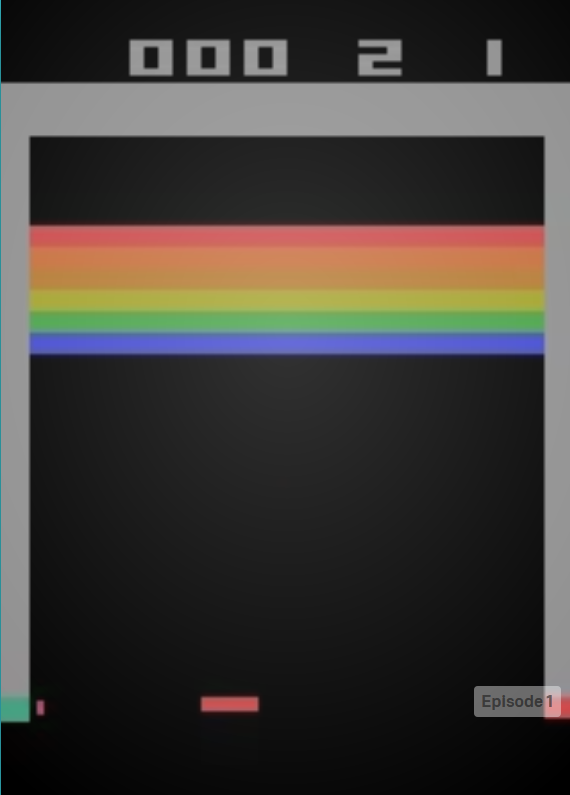
\includegraphics[width=\linewidth, height=0.2\textheight, keepaspectratio]{img/breakout.png}
    \caption{Sample Atari\texttrademark{} Breakout Game with Random Agent~\autocite{breakout}}~\label{fig:breakout}
\end{figure}


As previously mentioned for our term project, we wish to design and train a deep neural network that can play the nostalgic Atari\texttrademark{} Breakout game. The agent is expected to have an ``understanding'' of game mechanics such as how to score, and what moves to avoid. Essentially the agent is expected to have a functioning Atari\texttrademark{} skills.
A set of rewards and punishments, which are associated with certain in-game actions and outcomes, will be used to train the model who play the game over and over again.
At each epoch the artificial intelligence should be a better ``gamer'' than the previous one.

We are planning to conduct a research about reinforcement learning, deep neural networks and more specific algorithms like Deep Q-networks (DQN) that combines Q-learning with deep neural networks to let reinforcement learning to be applied to complex, high dimensional environments, like video games~\autocite{openai}. Furthermore, we are planning to obtain a working, playable version of the Breakout game which is suitable for training and testing our artificial agent.

\section{Work Done \& Reaming Work}
\subsection{Work Done}
In our proposal, we stated that we would conduct a research on reinforcement learning, deep neural networks and more specific algorithms like Deep Q-networks (DQN) that combines Q-learning with deep neural networks to let reinforcement learning to be  applied to complex, high dimensional environments, like video games~\autocite{openai}. We conducted the promised research to find the optimal approaches to the problem in hand. We informed ourselves on the basics of reinforcement learning and especially on Q-learning with DQN implementations. There are more recent solutions like DeepMind's \textit{Agent57}~\autocite{badia2020agent57} that can outperform DQN based solutions for atari games. However, these type of approaches are necessary for games that have a credit assignment problem, which means that if we choose an action, and we only win or lose hundreds of actions later, leaving us with no idea as to which of our actions led to this win or loss, making it difficult to learn from our actions. The chosen Breakout game is not that complex nor that far-fetched. Thus, our prior research concludes that DQN based solution will be more than sufficient to outperform the atari human benchmark for the Breakout game.

In addition to our background research, we declared that we would obtain a working, playable version of the Breakout game which is suitable for training and testing our artificial agent. In this context, we are utilizing \textit{OpenAI}'s ``Gym'' environments for the implementation of the Breakout atari game. Basically there are two versions of the Breakout game present as a Gym environment. One of the versions provides information of the RAM throughout the game~\autocite{breakout}, and the other provides 3-channel image for each frame throughout the game~\autocite{breakout_image}. Currently both versions of the Breakout game can be initiated from our implementation, and we will decide which one of these versions is the optimum for our case after some experimentation.

At this point of the project, we obtained a playable version of the Breakout game with an human agent, that we call the ``keyboard agent'' by utilizing the example provided in the \textit{GitHub} repo of \texttt{openai/gym}~\autocite{keyboard_agent}. With this aspect of the program, an human agent can play the Breakout atari game by using the keyboard. Version of the game, either RAM based or image based, and the game speed can be adjusted using CLI arguments. In addition to our playable version, we also managed to initialize an artificial agent based version which is suitable for training and testing. Currently, this agent only takes random actions from the action space. However, this environment is crucial for the remaining of the project, and the training and testing will be conducted on this environment, details are provided in the next section.

\subsection{Remaining Work}
At this point we have both RAM and image based Breakout atari game, with an artificial agent and keyboard controlled versions. Currently, artificial agent only takes random actions, but we are planning to thrive on obtaining an artificial agent that outperforms human benchmark. The environments for the reinforcement learning aspect of the project are built, and they are operating successfully. The remaining work is to generate DQN based solution to improve the performance of the artificial agent. In the light of our background research, we believe we can provide an elegant approach. Finally, our research unveils that we should obtain an artificial agent that meets our requirements approximately within 70-96 hours of training.

\section{Work Breakdown Structure}

\printbibliography{}

\begin{appendices}
    \section{Python Code}
    \begin{appendices}
    \section{Contribution}
    \begin{table}[h]
        \centering
        \caption{Task Sharing}\label{tab:task_sharing}
        \begin{tabular}{rl}\toprule
            \textbf{Student}   & \textbf{Task}                              \\\midrule
            Abdullah Arda Aşçı & Setting OpenAI, and developing             \\
                               & wrappers for \texttt{gym} environment.     \\
                               & Training \& testing with different         \\
                               & hyperparameters.                           \\
            \midrule
            Atahan Yorgancı    & Background research about RL               \\
                               & and DQN\@. Implementation of artificial    \\
                               & agent. Cloud based training training       \\
                               & \& testing with different hyperparameters. \\
            \midrule
            Alim Toprak Fırat  & Background research about RL               \\
                               & and Q-Learning. Training \& testing        \\
                               & with different hyperparameters.            \\
            \midrule
            Tuna Alikaşifoğlu  & Developing CLI for running, and            \\
                               & training using \texttt{gym} environment.   \\
                               & Implementation of DQN\@. Training \&       \\
                               & testing with different                     \\ \bottomrule
        \end{tabular}
    \end{table}
\end{appendices}
\end{appendices}

\end{document}
